%% Creator: Inkscape inkscape 0.92.5, www.inkscape.org
%% PDF/EPS/PS + LaTeX output extension by Johan Engelen, 2010
%% Accompanies image file 'Method.pdf' (pdf, eps, ps)
%%
%% To include the image in your LaTeX document, write
%%   \input{<filename>.pdf_tex}
%%  instead of
%%   \includegraphics{<filename>.pdf}
%% To scale the image, write
%%   \def\svgwidth{<desired width>}
%%   \input{<filename>.pdf_tex}
%%  instead of
%%   \includegraphics[width=<desired width>]{<filename>.pdf}
%%
%% Images with a different path to the parent latex file can
%% be accessed with the `import' package (which may need to be
%% installed) using
%%   \usepackage{import}
%% in the preamble, and then including the image with
%%   \import{<path to file>}{<filename>.pdf_tex}
%% Alternatively, one can specify
%%   \graphicspath{{<path to file>/}}
%% 
%% For more information, please see info/svg-inkscape on CTAN:
%%   http://tug.ctan.org/tex-archive/info/svg-inkscape
%%
\begingroup%
  \makeatletter%
  \providecommand\color[2][]{%
    \errmessage{(Inkscape) Color is used for the text in Inkscape, but the package 'color.sty' is not loaded}%
    \renewcommand\color[2][]{}%
  }%
  \providecommand\transparent[1]{%
    \errmessage{(Inkscape) Transparency is used (non-zero) for the text in Inkscape, but the package 'transparent.sty' is not loaded}%
    \renewcommand\transparent[1]{}%
  }%
  \providecommand\rotatebox[2]{#2}%
  \newcommand*\fsize{\dimexpr\f@size pt\relax}%
  \newcommand*\lineheight[1]{\fontsize{\fsize}{#1\fsize}\selectfont}%
  \ifx\svgwidth\undefined%
    \setlength{\unitlength}{570.14264693bp}%
    \ifx\svgscale\undefined%
      \relax%
    \else%
      \setlength{\unitlength}{\unitlength * \real{\svgscale}}%
    \fi%
  \else%
    \setlength{\unitlength}{\svgwidth}%
  \fi%
  \global\let\svgwidth\undefined%
  \global\let\svgscale\undefined%
  \makeatother%
  \begin{picture}(1,0.33852881)%
    \lineheight{1}%
    \setlength\tabcolsep{0pt}%
    \put(0,0){\includegraphics[width=\unitlength,page=1]{Method.pdf}}%
    \put(0.02521709,0.19628522){\color[rgb]{0,0,0}\makebox(0,0)[lt]{\lineheight{1.25}\smash{\begin{tabular}[t]{l}RGB\end{tabular}}}}%
    \put(0.20863678,0.29429478){\color[rgb]{0,0,0}\makebox(0,0)[lt]{\lineheight{0.5}\smash{\begin{tabular}[t]{l}HSV\\HSL\\LCh\\YCrCb\\XYZ\\Lab\\Luv\\YUV\\RGB\\OKLab\end{tabular}}}}%
    \put(0,0){\includegraphics[width=\unitlength,page=2]{Method.pdf}}%
    \put(0.58319412,0.19831426){\color[rgb]{0,0,0}\makebox(0,0)[lt]{\lineheight{1.25}\smash{\begin{tabular}[t]{l}Explainer\\\end{tabular}}}}%
    \put(0,0){\includegraphics[width=\unitlength,page=3]{Method.pdf}}%
    \put(0.81563653,0.31771241){\color[rgb]{0,0,0}\makebox(0,0)[lt]{\smash{\begin{tabular}[t]{l}Channel\\size\end{tabular}}}}%
    \put(2.74045852,0.18104435){\color[rgb]{0,0,0}\makebox(0,0)[lt]{\begin{minipage}{0.68449928\unitlength}\raggedright \end{minipage}}}%
    \put(0,0){\includegraphics[width=\unitlength,page=4]{Method.pdf}}%
    \put(0.42459295,0.32144212){\color[rgb]{0,0,0}\makebox(0,0)[lt]{\smash{\begin{tabular}[t]{l}SVM\end{tabular}}}}%
    \put(0,0){\includegraphics[width=\unitlength,page=5]{Method.pdf}}%
    \put(0.81444501,0.21047166){\color[rgb]{0,0,0}\makebox(0,0)[lt]{\lineheight{1.25}\smash{\begin{tabular}[t]{l}Model\\Selector\\\end{tabular}}}}%
    \put(0,0){\includegraphics[width=\unitlength,page=6]{Method.pdf}}%
    \put(0.96468934,0.20794801){\color[rgb]{0,0,0}\makebox(0,0)[lt]{\smash{\begin{tabular}[t]{l}Best\\Model\end{tabular}}}}%
    \put(0,0){\includegraphics[width=\unitlength,page=7]{Method.pdf}}%
    \put(0.14458949,0.02573369){\color[rgb]{0,0,0}\makebox(0,0)[t]{\lineheight{0.30000001}\smash{\begin{tabular}[t]{c}Data\\Preparation\end{tabular}}}}%
    \put(0.51453522,0.01269215){\color[rgb]{0,0,0}\makebox(0,0)[t]{\lineheight{0.30000001}\smash{\begin{tabular}[t]{c}X-AI Method\end{tabular}}}}%
    \put(0.8694959,0.02231761){\color[rgb]{0,0,0}\makebox(0,0)[t]{\lineheight{0.30000001}\smash{\begin{tabular}[t]{c}Model\\Selection\end{tabular}}}}%
  \end{picture}%
\endgroup%
